\subsection{第二型曲线积分}

	\begin{ti}
		设 $l$ 为自点 $O(0,0)$ 沿曲线 $y = \sin x$ 至点 $A(\uppi,0)$ 的有向弧段,求平面第二型曲线积分
		\[
			I = \int_{l} \bigl[ \ee^{x} \cos y + 2 (x + y) \bigr] \dd{x} + \Biggl( -\ee^{x} \sin y + \frac{3}{2}x \Biggr) \dd{y}.
		\]
	\end{ti}

	\begin{ti}
		设 $L$ 为圆周 $x^{2} + y^{2} = 4$ 正向一周,求
		\[
			I = \oint_{L} y^{3} \dd{x} + \bigl| 3y - x^{2} \bigr| \dd{y}.
		\]
	\end{ti}

	\begin{ti}
		计算曲线积分 $\oint_{L} \frac{y \dd{x} - x \dd{y}}{2\left(x^{2} + y^{2}\right)}$,其中 $L: (x - 1)^{2} + y^{2} = 2$,其方向为逆时针方向.
	\end{ti}

	\begin{ti}
		计算曲线积分 $\int_{C} \sqrt{x^{2} + y^{2}} \dd{x} + \bigl[ 2x + y\ln\bigl( x + \sqrt{x^{2} + y^{2}} \bigr) \bigr] \dd{y}$,其中有向曲线 $C: y = \sqrt{1 - \frac{(x - 3)^{2}}{4}}$,方向从点 $(5,0)$ 到点 $(1,0)$.
	\end{ti}

	\begin{ti}
		计算曲线积分
		\[
			\int_{L} \left( \frac{xy^{2}}{\sqrt{4 + x^{2}y^{2}}} + \frac{1}{\uppi}x \right)\dd{x} + \left( \frac{x^{2}y}{\sqrt{4 + x^{2}y^{2}}} - x + y \right)\dd{y},
		\]
		其中 $L$ 是摆线 $\begin{cases}
			x = a (t - \sin t),\\
			y = a (1 - \cos t)
		\end{cases} (a > 0)$ 上自 $O(0,0)$ 至 $A(2\uppi a,0)$ 的一段有向曲线弧.
	\end{ti}

	\begin{ti}
		计算曲线积分
		\[
			I = \int_{l} \bigl[ u_{x}'(x,y) + xy \bigr] \dd{x} + u_{y}'(x,y) \dd{y},
		\]
		其中 $l$ 是从点 $A(0,1)$ 沿曲线 $y = \frac{\sin x}{x}$ 到点 $B(\uppi,0)$ 的曲线段. $u(x,y)$ 在 $xOy$ 平面上具有二阶连续偏导数,且 $u(0,1) = 1$,$u(\uppi,0) = \uppi$.
	\end{ti}

	\begin{ti}
		设 $y' = f(x,y)$ 是一条简单封闭曲线 $L$(取正向),$f(x,y) \ne 0$,其所围区域记为 $D$,$D$ 的面积为 $1$,则 $I = \oint_{L} xf(x,y) \dd{x} - \frac{y}{f(x,y)} \dd{y} = $\htwo.
	\end{ti}

	\begin{ti}
		在过点 $O(0,0)$ 和 $A(\uppi,0)$ 的曲线族 $y = a \sin x$ $(a > 0)$ 中,求一条曲线 $L$,使沿该曲线从 $O$ 到 $A$ 的积分 $\int_{L} \bigl( 1 + y^{3} \bigr) \dd{x} + (2x + y) \dd{y}$ 的值最小.
	\end{ti}

	\begin{ti}
		证明
		\[
			\oint_{\varGamma} x f(y) \dd{y} - \frac{y}{f(x)} \dd{x} \geq 2\uppi,
		\]
		其中 $\varGamma$ 为圆周曲线 $(x - a)^{2} + (y - a)^{2} = 1 (a > 0)$ 正向,$f(x)$ 连续取正值.
	\end{ti}

	\begin{ti}
		设曲线积分 $\int_{L} \bigl[ f(x) - \ee^{x} \bigr] \sin y \dd{x} - f(x) \cos y \dd{y}$ 与路径无关,其中 $f(x)$ 具有一阶连续导数,且 $f(0) = 0$,则 $f(x)$ 等于\kuo.

		\twoch{$\frac{1}{2}\bigl( \ee^{-x} - \ee^{x} \bigr)$}{$\frac{1}{2}\bigl( \ee^{x} - \ee^{-x} \bigr)$}{$\frac{1}{2}\bigl( \ee^{x} + \ee^{-x} \bigr) - 1$}{$1 - \frac{1}{2}\bigl( \ee^{x} + \ee^{-x} \bigr)$}
	\end{ti}

	\begin{ti}
		已知曲线积分 $\int_{L} \bigl[ \ee^{x} \cos y + y f(x) \bigr] \dd{x} + \bigl( x^{3} - \ee^{x} \sin y \bigr) \dd{y}$ 与路径无关且 $f(x)$ 有连续的导数,则 $f(x) = $\htwo.
	\end{ti}

	\begin{ti}
		设 $f(x,y)$ 在全平面有连续偏导数,曲线积分 $\int_{L} f(x,y) \dd{x} + x \cos y \dd{y}$ 在全平面与路径无关,且 $\int_{(0,0)}^{\left(t,t^{2}\right)} f(x,y) \dd{x} + x \cos y \dd{y} = t^{2}$,求 $f(x,y)$.
	\end{ti}

	\begin{ti}
		设函数 $P(x,y) = \frac{x}{y}r^{\lambda}$,$Q(x,y) = - \frac{x^{2}}{y^{2}}r^{\lambda}$,其中 $r = \sqrt{x^{2} + y^{2}}$,若曲线积分 $\int_{L} P \dd{x} + Q \dd{y}$ 在区域 $D = \bigl\{ (x,y) \bigl| y > 0 \bigr\}$ 上与路径无关,求参数 $\lambda$.
	\end{ti}

	\begin{ti}
		设 $L$ 是摆线 $\begin{cases}
			x = t - \sin t - \uppi,\\
			y = 1 - \cos t
		\end{cases}$ 从 $t = 0$ 到 $t = 2\uppi$ 的一段,则 $\int_{L} \frac{(x - y)\dd{x} + (x + y) \dd{y}}{x^{2} + y^{2}} = $\kuo.
		
		\fourch{$-\uppi$}{$\uppi$}{$2\uppi$}{$-2\uppi$}
	\end{ti}

	\begin{ti}
		设函数 $g(x)$ 具有连续导数,曲线积分
		\[
			\int_{L} \bigl[ \ee^{2x} + g'(x) - 2g(x) \bigr]y \dd{x} - g'(x) \dd{y}
		\]
		与路径无关.
		\begin{enumerate}
			\item 求满足条件 $g(0) = -\frac{1}{4}, g'(0) = -\frac{1}{2}$ 的函数 $g(x)$;
			\item 计算 $\int_{(0,0)}^{(1,1)} \bigl[ \ee^{2x} + g'(x) - 2g(x) \bigr]y \dd{x} - g'(x) \dd{y}$ 的值.
		\end{enumerate}
	\end{ti}

	\begin{ti}
		微分方程 $\bigl( 2xy + \ee^{x}\sin y \bigr) \dd{x} + \bigl( x^{2} + \ee^{x} \cos y \bigr) \dd{y} = 0$ 的通解为\htwo.
	\end{ti}

	\begin{ti}
		\begin{enumerate}
			\item 设函数 $f(x)$ 具有一阶连续导数,且 $f(1) = 1$,$D$ 为不包含原点的单连通区域,在 $D$ 内曲线积分 $\int_{L} \frac{y\dd{x} - x\dd{y}}{2x^{2} + f(y)}$ 与路径无关,求 $f(y)$;\label{7.46:1}
			\item 在(\ref{7.46:1})的条件下,求 $\oint_{L'} \frac{y\dd{x} - x\dd{y}}{2x^{2} + f(y)}$,其中 $L'$ 为曲线 $x^{\frac{2}{3}} + y^{\frac{2}{3}} = a^{\frac{2}{3}}, a > 0$,且取逆时针方向.
		\end{enumerate}
	\end{ti}

	\begin{ti}
		设 $L$ 为曲线 $x^{2} + y^{2} = R^{2}$(常数 $R > 0$)一周,$\bm n$ 为 $L$ 的外法线方向向量,$u(x,y)$ 具有二阶连续偏导数且 $\frac{\partial^{2}u}{\partial x^{2}} + \frac{\partial^{2}u}{\partial y^{2}} = x^{2} + y^{2}$. 求 $\oint_{L} \frac{\partial u}{\partial \bm n} \dd{s}$.
	\end{ti}

	\begin{ti}
		计算 $\int_{\varGamma} y\dd{x} + z\dd{y} + x\dd{z}$,其中 $\varGamma$ 为螺旋线 $x = a \cos t, y = a \sin t, z = bt$ 从 $t = 0$ 到 $t = 2\uppi$ 的一段,如图~\ref{fig:1.7.3} 所示.
		\begin{figure}[htbp]
			\centering
			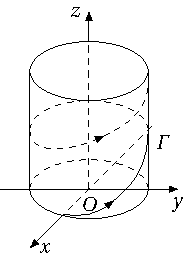
\includegraphics[scale=1]{figure/fig1-7-3.pdf}
			\caption{}\label{fig:1.7.3}
		\end{figure}
	\end{ti}